\chapter{The Gaussian Distribution and Quantiles}
\label{ch:gaussian}

\begin{chaptergoals}
\begin{itemize}[nosep]
\item The Gaussian density: what each piece of the formula does, why the CDF has no closed form, and why the tails are so thin that the distribution lives in a finite interval for practical purposes.
\item The three properties used constantly from here on: closure under affine transformations, standardization, and symmetry. Plus the one that usually goes unstated: sums of independent Gaussians are Gaussian.
\item How to turn a Gaussian probability into a table lookup, forwards and backwards.
\item Quantiles, in this book's convention $q_\alpha$ (the number with mass $\alpha$ to its \textit{right}), the four values worth memorizing, and the one-sided versus two-sided distinction that every confidence interval and test depends on.
\end{itemize}
This chapter is a review. If you know it, read the quantile section for the notation and move on.
\end{chaptergoals}

\section{Why the Gaussian is everywhere}
\label{sec:gauss-why}

\Cref{ch:lln,ch:clt,ch:limit-tools} kept producing Gaussian limits; this chapter collects what you need about the Gaussian to use them, and fixes the quantile notation of the rest of the book.
Because of the Central Limit Theorem (\cref{ch:clt}), the Gaussian (also called the normal) distribution is ubiquitous in statistics: every average of enough independent, identically distributed draws with finite variance is approximately Gaussian, whatever the draws come from, so every estimator built from an average inherits a Gaussian error distribution for large $n$.
That is where the Gaussian enters statistical inference, and it stays: confidence intervals, test statistics, the asymptotic distribution of the maximum likelihood estimator, the error term of linear regression.
The distribution is named after Carl Friedrich Gauss (1777--1855), who arrived at it in the context of the method of least squares, which is the subject of \cref{ch:regression-uni}.

\section{The density and its CDF}
\label{sec:gauss-density}

\begin{definition}[Gaussian distribution]
\label{def:gaussian}
A continuous r.v.\ $X$ has the \textbf{Gaussian distribution} with parameters $\mu \in \real$ and $\sigma^2 > 0$ if its PDF is given by:
\[
f_{\mu, \sigma^2}(x) = \frac{1}{\sigma \sqrt{2 \pi}} \exp \left(- \frac{(x - \mu)^2}{2 \sigma^2} \right), \, \text{ for } x \in (-\infty, \infty).
\]
You write this as $X \sim \Gauss(\mu, \sigma^2)$, and then $\E[X] = \mu$ and $\var(X) = \sigma^2$.
The case $\mu = 0$, $\sigma^2 = 1$ is the \textbf{standard Gaussian}, whose density and CDF get their own letters:
\[
\varphi(z) = \frac{1}{\sqrt{2\pi}} e^{-z^2/2}, \qquad \Phi(z) = \int_{-\infty}^z \varphi(t) \, \mathrm{d}t.
\]
\end{definition}

\begin{inwords}
\textbf{In words.} A Gaussian variable is one whose probabilities are areas under the bell-shaped curve above \toolkit{sec:math-density}; $\mu$ says where the bell is centered and $\sigma$ how wide it is. Two numbers fix the whole distribution.
\par\smallskip
\textbf{For the kiss data.} The CLT says $\bar{R}_n$ behaves, for large $n$, like a Gaussian with $\mu = p$ and $\sigma^2 = p(1-p)/n$: centered at the truth, with width $0.043$ at $n = 124$ and $p = 0.645$.
\end{inwords}

Take the formula apart.
The constant $\ds \frac{1}{\sigma \sqrt{2 \pi}}$ is a \textit{normalizing constant}: it normalizes the total area under the PDF to 1, and plays no other role.
Everything about the shape is in the exponent.
Consider the quadratic there:
\[
- \frac{(x - \mu)^2}{2\sigma^2} = - \left( \frac{x^2 - 2\mu x + \mu^2}{2\sigma^2} \right).
\]
It is zero at $x = \mu$ and negative everywhere else, so the density peaks at $\mu$ and falls off symmetrically on both sides.
If $\sigma$ is small, that is, if the standard deviation is small, then the quadratic is more negative at the same distance from $\mu$, so the exponential falls off faster and the density is narrower.
A small standard deviation and a narrow density are the same thing seen twice.
\Cref{fig:gaussdensity} shows the effect of each parameter.
On the left, $\Gauss(0, 4)$ is $\Gauss(0, 1)$ stretched to twice the width, and its peak drops to half the height to keep the area at $1$; $\Gauss(10, 4)$ is $\Gauss(0, 4)$ moved ten units to the right with no change of shape.
So $\mu$ moves the density without changing its shape, and $\sigma$ stretches it without moving its center.
On the right, the three shaded regions of the standard Gaussian have probabilities $0.6827$, $0.9545$ and $0.9973$: the `$68$--$95$--$99.7$ rule' of an introductory course, stated exactly.

\begin{figure}[htbp]
\centering
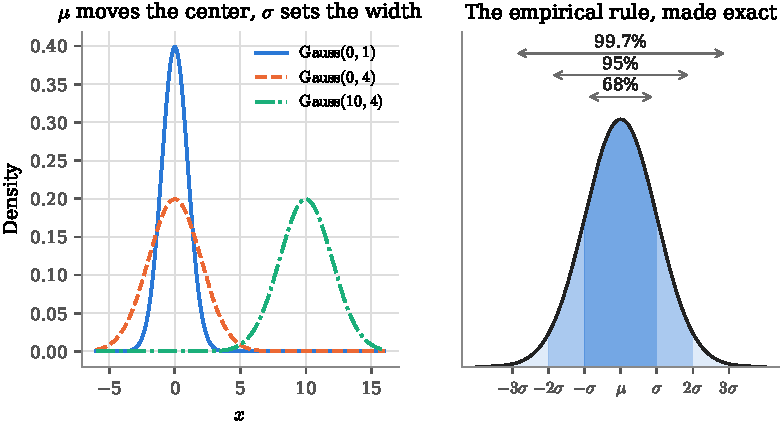
\includegraphics[width=\textwidth]{fig_gaussian_density}
\caption{Left: the densities of $\Gauss(0, 1)$ (solid), $\Gauss(0, 4)$ (dashed) and $\Gauss(10, 4)$ (dash-dot). Right: the standard Gaussian density, shaded within one, two and three standard deviations of the mean.}
\label{fig:gaussdensity}
\end{figure}

Two consequences of the exponent are worth stating on their own.
\begin{itemize}
\item \textbf{The tails are thin.}
The density decays like $e^{-x^2/(2\sigma^2)}$, faster than any exponential $e^{-c|x|}$, so for practical purposes a Gaussian lives in a finite interval: $99.7\%$ of the mass is within $3\sigma$ of $\mu$, and the probability of being more than $5\sigma$ away is about one in two million.
This is what licenses a statement like `with overwhelming probability $\abs{\bar{X}_n - \mu} \leq 3\sigma/\sqrt{n}$' (\cref{sec:clt}).
\item \textbf{The CDF has no closed form.}
\[
\Pr(X \leq x) = F_{\mu, \sigma^2}(x) = \frac{1}{\sigma \sqrt{2\pi}} \int_{-\infty}^x \exp \left(- \frac{(t - \mu)^2}{2 \sigma^2} \right) \, \mathrm{d}t
\]
must be left as an integral: it's mathematically impossible to write the antiderivative of $e^{-t^2/2}$ in terms of elementary functions.
Still, $F_{\mu, \sigma^2}$ is a perfectly well-defined function: input some value $x$ and it returns the accumulated area under the PDF from $-\infty$ up to $x$.
You get its values from tables or from software, and \cref{sec:gauss-computing} says how.
\end{itemize}

\section{Properties of Gaussian distributions}
\label{sec:gauss-properties}

\begin{enumerate}
\item \textbf{Affine transformation.}
Perhaps the most useful property of the Gaussian family is that it is invariant under affine transformations.
Given the r.v.\ $X \sim \Gauss(\mu, \sigma^2)$, then
\[
aX + b \sim \Gauss(a\mu + b, a^2\sigma^2) \qquad \text{for all } a \neq 0, \, b \in \real.
\]
Shifting and rescaling a Gaussian produces another Gaussian; the mean and variance change in the way means and variances always do under $aX + b$, and the shape stays Gaussian, which is the content of the statement.

\optionalproof{Write the CDF of $aX + b$ as a CDF of $X$ at a transformed point, differentiate (chain rule) to get the density, and recognize the Gaussian formula with new parameters \toolkit{sec:math-density}.}
\begin{proof}
Take $a > 0$ (the case $a < 0$ is the same with the inequality flipped).
The CDF of $Y = aX + b$ is
\[
F_Y(y) = \Pr(aX + b \leq y) = \Pr \left( X \leq \frac{y - b}{a} \right) = F_X \left( \frac{y-b}{a} \right).
\]
Differentiate with respect to $y$ (chain rule) to get the density:
\begin{align*}
f_Y(y) = \frac{1}{a} f_X \left( \frac{y - b}{a} \right) &= \frac{1}{a \sigma \sqrt{2\pi}} \exp \left( - \frac{\left( \frac{y-b}{a} - \mu \right)^2}{2 \sigma^2} \right) \\
&= \frac{1}{(a\sigma) \sqrt{2\pi}} \exp \left( - \frac{(y - (a\mu + b))^2}{2 (a\sigma)^2} \right),
\end{align*}
which is the $\Gauss(a\mu + b, a^2 \sigma^2)$ density.
\end{proof}

\item \textbf{Standardization.}
If $X \sim \Gauss(\mu, \sigma^2)$, then:
\[
Z = \frac{X - \mu}{\sigma} \sim \Gauss(0, 1).
\]
This is the affine property with $a = 1/\sigma$ and $b = -\mu/\sigma$, and it is the single most used fact about the Gaussian because it reduces every Gaussian probability to a probability about the one fixed distribution that is tabulated.
That is because of standardization, you have that:
\[
\Pr(u \leq X \leq v) = \Pr \left( \frac{u - \mu}{\sigma} \leq Z \leq \frac{v-\mu}{\sigma}\right) = \Phi \left( \frac{v-\mu}{\sigma} \right) - \Phi \left( \frac{u-\mu}{\sigma} \right),
\]
where $Z$ on the right-hand side is as above, $Z = \frac{X - \mu}{\sigma}$.

\textbf{Question:} Why does this last result follow?

\textbf{Answer:} Consider $\Pr(u \leq X \leq v)$ where $X \sim \Gauss(\mu, \sigma^2)$.
First, mean-center the variables by subtracting the mean of $X$ in the inequalities and then divide each term by the standard deviation.
\begin{align*}
\Pr(u \leq X \leq v) &= \Pr(u - \mu \leq X - \mu \leq v - \mu) \\
					 &= \Pr \left( \frac{u - \mu}{\sigma} \leq \frac{X - \mu}{\sigma} \leq \frac{v - \mu}{\sigma} \right) \\
					 &= \Pr \left( \frac{u - \mu}{\sigma} \leq Z \leq \frac{v - \mu}{\sigma} \right).
\end{align*}
Observe that the inequalities are preserved because adding a number and multiplying by a positive number doesn't change an inequality's direction.

\item \textbf{Symmetry.}
If $X \sim \Gauss(0, \sigma^2)$, then $-X \sim \Gauss(0, \sigma^2)$ (the affine property with $a = -1$, $b = 0$).
Consequently, for $x > 0$:
\begin{align*}
\Pr(\abs{X} > x) &= \Pr(X > x \text{ or } X < -x) \\
				&= \Pr(X > x) + \Pr(X < -x) \\
				&= \Pr(X > x) + \Pr(-X > x) \\
				&= 2 \Pr(X > x).
\end{align*}
Intuitively, when you negate a Gaussian r.v.\ you mirror its distribution about the vertical axis.
This mirroring doesn't change the shape or the spread of the distribution; it only changes the sign of the values.
As a result, the negated Gaussian random variable $-X$ maintains the same mean (here, 0) and the same variance $\sigma^2$ as the original r.v.\ $X$.
For the standard Gaussian the symmetry reads $\Phi(-z) = 1 - \Phi(z)$, which is why tables only print positive $z$.

\item \textbf{Sums of independent Gaussians are Gaussian.}
If $X_1 \sim \Gauss(\mu_1, \sigma_1^2)$ and $X_2 \sim \Gauss(\mu_2, \sigma_2^2)$ are independent, then
\[
X_1 + X_2 \sim \Gauss(\mu_1 + \mu_2, \sigma_1^2 + \sigma_2^2).
\]
The mean and variance are what they would be for any independent pair; the point is again that the shape stays Gaussian.
(The proof is omitted here; it follows from the convolution formula, or in one line from moment generating functions.)
Combined with the affine property, it gives the fact behind every exact small-sample result in this book: if $\Xton \iid \Gauss(\mu, \sigma^2)$ then
\[
\bar{X}_n \sim \Gauss \left( \mu, \frac{\sigma^2}{n} \right) \qquad \text{exactly, for every } n,
\]
with no appeal to the Central Limit Theorem.
For Gaussian data the CLT's conclusion holds at $n = 2$.
\end{enumerate}

\begin{bridge}[$z$-scores]
Standardization is the $z$-score of an introductory course: `how many standard deviations above the mean is this observation?'
What the introductory course sometimes leaves unsaid is that the $z$-score of a Gaussian observation is itself a standard Gaussian random variable, which is the reason a single table serves every $\mu$ and $\sigma$.
Here the same move is applied not to an observation but to an estimator: $\sqrt{n}(\bar{X}_n - \mu)/\sigma$ is the $z$-score of $\bar{X}_n$, and the CLT says it is approximately standard Gaussian.
Every `$z$-interval' and `$z$-test' you learned is that sentence plus a quantile from \cref{sec:gauss-quantiles}.
\end{bridge}

\section{Computing probabilities, forwards and backwards}
\label{sec:gauss-computing}

Since the CDF has no formula, every Gaussian probability is computed by standardizing and then looking up $\Phi$, in a table or in software.
There are two directions.
\textit{Forwards:} given a value, find a probability; standardize to a $z$-score and read $\Phi(z)$.
\textit{Backwards:} given a probability, find the value; read the table in reverse to get $z = \Phi^{-1}(\text{probability})$ and unstandardize, $x = \mu + \sigma z$.
\Cref{fig:gausscdf} shows both on the graph of $\Phi$, with the numbers of the exam example that follows.
Forwards, a $z$-score goes in on the horizontal axis and a probability comes out on the vertical axis: $\Phi(2.5) = 0.9938$.
Backwards, a probability goes in on the vertical axis and a $z$-score comes out on the horizontal axis: $\Phi^{-1}(0.90) = 1.28$.
Tables print the forward direction; for the backward direction you scan the table for the probability, or ask software for the quantile directly.

\begin{figure}[htbp]
\centering
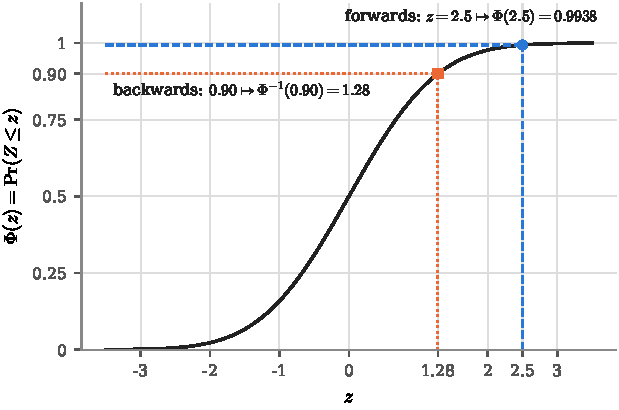
\includegraphics[width=0.72\textwidth]{fig_gaussian_cdf}
\caption{The standard Gaussian CDF $\Phi$ with the two readings of the exam example below: forwards from $z = 2.5$ to $\Phi(2.5) = 0.9938$ (blue dashes), backwards from $0.90$ to $\Phi^{-1}(0.90) = 1.28$ (orange dots).}
\label{fig:gausscdf}
\end{figure}

\begin{worked}[exam scores]
Assume that the score distribution for a final exam is approximately $X \sim \Gauss(85, 4)$, that is, mean $85$ and standard deviation $\sigma = 2$.
\begin{itemize}[nosep]
\item $\Pr(X > 90)$. Standardize: $z = (90 - 85)/2 = 2.5$. Then $\Pr(X > 90) = \Pr(Z > 2.5) = 1 - \Phi(2.5) = 1 - 0.9938 = 0.0062$. About six students in a thousand score above $90$.
\item $\Pr(80 < X < 90)$. The endpoints standardize to $-2.5$ and $2.5$, so $\Pr(80 < X < 90) = \Phi(2.5) - \Phi(-2.5) = 2\Phi(2.5) - 1 = 0.9876$, using the symmetry $\Phi(-z) = 1 - \Phi(z)$.
\item The score $x$ such that $\Pr(X < x) = 0.90$ (the $90$th percentile). For this you read the table backwards: the $z$ with $\Phi(z) = 0.90$ is $z = 1.2816$, so $x = 85 + 2 \times 1.2816 = 87.6$.
\end{itemize}
\end{worked}

\begin{pitfall}[variance or standard deviation?]
This book writes $\Gauss(\mu, \sigma^2)$: the second parameter is the \textit{variance}.
So $\Gauss(85, 4)$ has standard deviation $2$, and $\Gauss(10, 4)$ in \cref{fig:gaussdensity} is twice as wide as $\Gauss(0, 1)$, not four times.
Most software and many textbooks take the standard deviation instead, and the mix-up fails silently: for the exam scores, $\Pr(X \leq 90)$ is $0.994$ with standard deviation $2$, but a $4$ entered where the $2$ was meant answers a different question and gives $0.894$, with no warning that anything went wrong.
Check which convention is in force every time, and when you write $\Gauss(\mu, \sigma^2)$ yourself, write the square.
\end{pitfall}

\section{Quantiles}
\label{sec:gauss-quantiles}

To grasp the idea of a quantile it's instructive to consider an example involving a closely related idea, a percentile.
Suppose you score a 72 on an exam.
Then your percentile is the fraction of students who score \textit{below} a 72.
In terms of probability, percentiles are computed using the CDF of exam scores: Letting $X$ denote the score of a random student on the exam, and to make things easy supposing $X$ is a continuous r.v., then your percentile is $\Pr(X \leq 72) = F_X(72)$.

In general, a student with score $x$ has percentile $F_X(x)$.
Going the other way, if you start with a percentile, say $0.95$, then $F^{-1}(0.95)$ is the score on the exam that has that percentile.
A percentile is also called a quantile, which is why $F^{-1}$ is called the \textbf{quantile function}.\footnote{More precisely, a percentile is a quantile expressed as a percentage.}
The function $F$ converts scores to quantiles, and the function $F^{-1}$ converts quantiles to scores: the forward and backward readings of \cref{fig:gausscdf}.
And finally, note that a quantile (of a specific order) is a number in the support of an r.v., not a probability.
Now for the formal definition, in the convention this book uses throughout.

\begin{definition}[Quantile of order $1 - \alpha$]
\label{def:quantile}
Let $\alpha \in (0,1)$.
The \textbf{quantile of order $1 - \alpha$} of an r.v.\ $X$ is the number $q_\alpha$ such that
\[
\Pr(X \leq q_\alpha) = 1 - \alpha.
\]
\end{definition}

\begin{figure}[htbp]
\centering
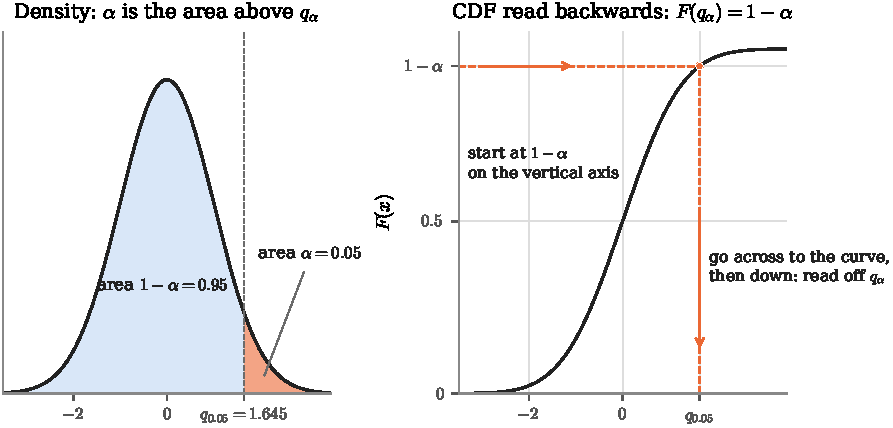
\includegraphics[width=\textwidth]{fig_quantile_def}
\caption{The definition of $q_\alpha$ for the standard Gaussian, $\alpha = 0.05$. Left: the density, with area $1 - \alpha$ below $q_\alpha$ (blue) and area $\alpha$ above it (orange). Right: the CDF, with the backward reading from $1 - \alpha$ to $q_\alpha$ (orange dashes).}
\label{fig:quantiledef}
\end{figure}

\begin{inwords}
\textbf{In words.} $q_\alpha$ is the cutoff with probability $\alpha$ above it and $1 - \alpha$ below: read the CDF backwards at $1 - \alpha$, as in \cref{fig:quantiledef} \toolkit{sec:math-density}. The subscript names the tail it cuts off, so read $q_{0.05}$ as `the cutoff with $5\%$ above it'.
\par\smallskip
\textbf{For the kiss data.} The $1.96$ in $\bar{R}_n \pm 1.96 \times 0.043$ is $q_{0.025}$: it leaves $2.5\%$ in each tail, $5\%$ in both, so the interval catches the standardized error $95\%$ of the time.
\end{inwords}

\textbf{How to read the notation.}
The symbol $q_\alpha$ carries two numbers and it is easy to attach the subscript to the wrong one.
The subscript $\alpha$ is a \textit{probability}, the area of the upper tail in \cref{fig:quantiledef}; the value $q_\alpha$ is a \textit{number on the horizontal axis}, a cutoff in the same units as $X$.
The left of the figure shows the first as a shaded area and the second as the cutoff that leaves area $\alpha$ to its right and $1 - \alpha$ to its left.
The right shows how to find the cutoff: read the CDF backwards, starting at height $1 - \alpha$ on the vertical axis, going across to the curve, then dropping down to the horizontal axis; the number you land on is $q_\alpha$, and for the standard Gaussian and $\alpha = 0.05$ it is $1.645$.
So $q_{0.05} = 1.645$ says: the probability that a standard Gaussian exceeds $1.645$ is $0.05$.
The phrase `quantile of order $1 - \alpha$' in the definition refers to the area \textit{below} the cutoff, $0.95$ for $q_{0.05}$, which is how the inverse CDF is indexed; the subscript refers to the area \textit{above}.
Both describe the same point.

\textbf{Remark:} It might seem weird to define quantiles in terms of their complements;
that is, the quantile is of order $1 - \alpha$ and not of order $\alpha$.
The reason is what the quantile is for.
In the formulas that follow, $\alpha$ is usually a small tail probability (a $5\%$ level, a $2.5\%$ tail), and $q_\alpha$ is the cutoff that leaves exactly that much probability in the upper tail.
Indexing the cutoff by the tail it cuts off, rather than by the mass below it, is what makes $q_{0.05}$ mean `the $5\%$ critical value' in every formula that follows.
In an intro course the same number arrived as $z^* = 1.645$ or $z_{0.05}$ from the back of the book; $q_{0.05}$ is that $z^*$ with the tail it cuts off written into the name.

\textbf{Properties of quantiles.}
In the following let $F$ be the CDF of some r.v.\ $X$, assumed continuous and strictly increasing so that $F^{-1}$ exists.
\begin{itemize}
\item By the definitions of CDFs and quantiles, it follows that $F(q_{\alpha}) = 1 - \alpha$.
\item How do you find $q_{\alpha}$, the quantile of order $1-\alpha$?
Since $F(q_{\alpha}) = 1 - \alpha$, you just take the inverse of $F$, meaning $F^{-1}(1-\alpha) = q_{\alpha}$.
\item Note also that $\Pr(X > q_{\alpha}) = \alpha$.
This follows from the definition of quantiles by considering the complement of $\Pr(X \leq q_{\alpha})$, and it's the form you'll use most: $q_\alpha$ is the number exceeded with probability $\alpha$.
\item Let $X = Z \sim \Gauss(0,1)$.
Then $\alpha$ equals the probability that $\abs{Z}$ is greater than $q_{\alpha/2}$.
That is, $\Pr(\abs{Z} > q_{\alpha/2}) = \alpha$.
This is the symmetry property: $\Pr(\abs{Z} > q_{\alpha/2}) = 2\Pr(Z > q_{\alpha/2}) = 2 \cdot \alpha/2$.
\end{itemize}

The last property is the two-sided version, and the difference between it and the one-sided definition is drawn in \cref{fig:gaussquantiles}.
For a one-sided statement (`$Z$ exceeds the cutoff') the cutoff is $q_\alpha$; for a two-sided statement (`$Z$ is beyond the cutoff in either direction') the cutoff is $q_{\alpha/2}$ because the probability $\alpha$ has to be split between two tails.
With $\alpha = 0.05$: on the left of the figure, $q_{0.05} = 1.645$ leaves $5\%$ of the mass in the upper tail; on the right, $q_{0.025} = 1.96$ leaves $2.5\%$ in each tail, so $\abs{Z} > 1.96$ has probability $5\%$.
Same $\alpha$, different cutoff.

\begin{figure}[htbp]
\centering
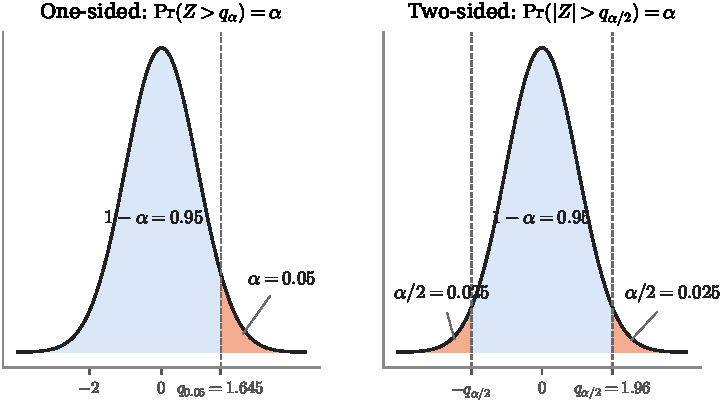
\includegraphics[width=\textwidth]{fig_gaussian_quantiles}
\caption{The standard Gaussian density with $\alpha = 0.05$. Left: the one-sided cutoff $q_{0.05} = 1.645$, with the tail of area $0.05$ in orange. Right: the two-sided cutoffs $\pm q_{0.025} = \pm 1.96$, with the two tails of area $0.025$ each in orange.}
\label{fig:gaussquantiles}
\end{figure}

Some important quantiles of the standard Gaussian, which recur so often that it is worth knowing them by heart:
\begin{center}
\begin{tabular}{@{}lcccc@{}}
\toprule
$\alpha$ & $10\%$ & $5\%$ & $2.5\%$ & $0.5\%$ \\
\midrule
$q_\alpha$ & $1.28$ & $1.645$ & $1.96$ & $2.576$ \\
\bottomrule
\end{tabular}
\end{center}
Read across: $\Pr(Z > 1.28) = 10\%$, $\Pr(Z > 1.645) = 5\%$, $\Pr(Z > 1.96) = 2.5\%$, $\Pr(Z > 2.576) = 0.5\%$.
And read two-sided: $\Pr(\abs{Z} > 1.645) = 10\%$, $\Pr(\abs{Z} > 1.96) = 5\%$, $\Pr(\abs{Z} > 2.576) = 1\%$.
The $1.96$ of every $95\%$ confidence interval is $q_{0.025}$, not $q_{0.05}$.

\begin{pitfall}[which $\alpha$ is that?]
Two conventions collide here and both are in common use.
This book's $q_\alpha$ has mass $\alpha$ \textit{above} it: $q_{0.05} = 1.645$.
Software and many textbooks index a quantile by the mass \textit{below} it: on that convention the $0.95$-quantile is $1.645$ and the $0.05$-quantile is $-1.645$.
So this book's $q_\alpha$ is the other convention's $(1 - \alpha)$-quantile, and its $q_{\alpha/2}$ for a $95\%$ interval is the other convention's $0.975$-quantile.
When a formula in this book says $q_{\alpha/2}$ and you reach for a table or software that counts from below, look up $1 - \alpha/2$.
\Cref{fig:quantiledef} is the picture to keep in mind: the subscript is the area in the upper tail.
\end{pitfall}

\begin{example}[Quantiles of the Exponential]
\label{ex:expo-quantile}
Let $X \sim \Expo(\lambda)$, with CDF $F_X(x) = 1 - e^{-\lambda x}$ for $x \geq 0$.
To find the number $x$ below which the mass is $p$, solve $F_X(x) = p$:
\begin{align*}
1 - e^{-\lambda x} &= p \\
e^{-\lambda x} &= 1 - p \\
-\lambda x &= \ln(1 - p) \\
x &= -\frac{\ln(1-p)}{\lambda}.
\end{align*}
So, for example, the 50th percentile, or median, of an Exponential r.v.\ with parameter $\lambda$ is $x = -\ln(1/2)/\lambda = \ln 2 / \lambda \approx 0.69/\lambda$, which is less than the mean $1/\lambda$ because the distribution is skewed to the right.
In this book's notation, $q_\alpha = -\ln(\alpha)/\lambda$: the subway inter-arrival time of \cref{ch:limit-tools}, with $\hat{\lambda} = 0.16$ per minute, exceeds $q_{0.05} = -\ln(0.05)/0.16 \approx 19$ minutes about one time in twenty.
\Cref{fig:expoquantile} shows the three numbers on the density.
The median, $\ln 2/\lambda = 4.3$ minutes, splits the mass in half and sits left of the mean of $1/\lambda = 6.2$ minutes because the long right tail pulls the mean up; the quantile $q_{0.05} = 18.7$ minutes leaves $5\%$ of the mass above it.
For the Gaussian the median and the mean coincide; for a skewed distribution they don't.
\end{example}

\begin{figure}[htbp]
\centering
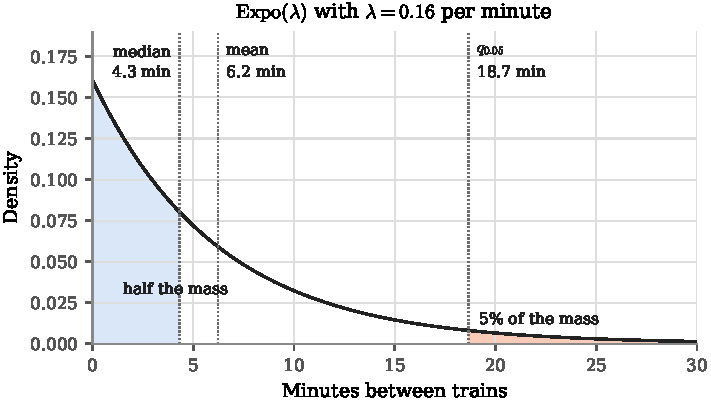
\includegraphics[width=0.8\textwidth]{fig_expo_quantile}
\caption{The $\Expo(\lambda)$ density of the subway inter-arrival times, $\lambda = 0.16$ per minute, with the median, the mean and $q_{0.05}$ marked by dotted lines. The half of the mass below the median is blue; the $5\%$ above $q_{0.05}$ is orange.}
\label{fig:expoquantile}
\end{figure}

\section{What comes next}
\label{sec:gauss-next}

This closes the probability part of the book.
Part III turns the three questions of \cref{ch:kiss} into definitions with guarantees, stated for the general model of \cref{ch:models}: \cref{ch:estimators} says what an estimator is and how to judge one; \cref{ch:confidence-intervals} and \cref{ch:tests-foundations} attach the two kinds of guarantee, an interval and a decision.
The Gaussian quantiles of this chapter appear in every formula of the last two.

\section{Summary}
\label{sec:gauss-summary}

\begin{itemize}[nosep]
\item $X \sim \Gauss(\mu, \sigma^2)$ has density $\frac{1}{\sigma\sqrt{2\pi}} \exp(-(x-\mu)^2/(2\sigma^2))$. The second parameter is the variance. The CDF has no closed form; the tails are thin enough that $3\sigma$ contains $99.7\%$ of the mass.
\item Affine transformations, in particular standardization $Z = (X - \mu)/\sigma \sim \Gauss(0,1)$, preserve Gaussianity; so do sums of independent Gaussians. The sample mean of Gaussian data is exactly $\Gauss(\mu, \sigma^2/n)$.
\item Every Gaussian probability is a table lookup after standardization: forwards for probabilities, backwards for quantiles. $\Phi(-z) = 1 - \Phi(z)$.
\item The quantile $q_\alpha$ of order $1 - \alpha$ satisfies $\Pr(X > q_\alpha) = \alpha$. For the standard Gaussian, $\Pr(\abs{Z} > q_{\alpha/2}) = \alpha$. Memorize $q_{0.05} = 1.645$ and $q_{0.025} = 1.96$, and keep straight which one a question needs.
\end{itemize}

\section{Exercises}
\label{sec:gauss-exercises}

\begin{exercise}
Let $Z \sim \Gauss(0,1)$. Compute $\Pr(Z \leq 1)$, $\Pr(Z \geq -1)$ and $\Pr(\abs{Z} > 1)$.
\end{exercise}
\begin{solution}
From the table, $\Phi(1) = 0.8413$. By symmetry $\Pr(Z \geq -1) = \Pr(Z \leq 1) = 0.8413$, and $\Pr(\abs{Z} > 1) = 2(1 - \Phi(1)) = 0.3173$. So about a third of standard Gaussian draws fall more than one standard deviation from the mean, the complement of the $68\%$ in \cref{fig:gaussdensity}.
\end{solution}

\begin{exercise}
Let $X \sim \Gauss(\mu, \sigma^2)$ and $Y = 2X$. Write down the PDF of $Y$, first from the affine property and then by the change-of-variables formula $f_Y(y) = f_X(g^{-1}(y)) / \abs{g'(g^{-1}(y))}$ for $Y = g(X)$.
\end{exercise}
\begin{solution}
By the affine property $Y \sim \Gauss(2\mu, 4\sigma^2)$, so $f_Y(y) = \frac{1}{2\sigma\sqrt{2\pi}} \exp \left( -\frac{(y - 2\mu)^2}{2 \cdot 4\sigma^2} \right)$. By change of variables with $g(x) = 2x$, $g^{-1}(y) = y/2$ and $g' = 2$: $f_Y(y) = \frac{1}{2} f_X(y/2) = \frac{1}{2\sigma\sqrt{2\pi}} \exp \left( -\frac{(y/2 - \mu)^2}{2\sigma^2} \right)$, and $(y/2 - \mu)^2 / (2\sigma^2) = (y - 2\mu)^2 / (8\sigma^2)$, the same thing.
\end{solution}

\begin{exercise}
Let $X \sim \Gauss(2, 2)$ (mean $2$, variance $2$) and let $x > 0$. Write $\Pr(X \geq -x)$ as $\Phi(g(x))$ for a function $g$ that is positive for $x > 0$.
\end{exercise}
\begin{solution}
Standardize: $(X - 2)/\sqrt{2} \sim \Gauss(0,1)$, so $\Pr(X \geq -x) = \Pr \left( Z \geq \frac{-x - 2}{\sqrt{2}} \right) = 1 - \Phi \left( -\frac{x+2}{\sqrt{2}} \right) = \Phi \left( \frac{x + 2}{\sqrt{2}} \right)$ by symmetry. For $x = 1$ this is $\Phi(2.12) = 0.983$.
\end{solution}

\begin{exercise}
Verify the three numbers of the empirical rule from a table, and find $\Pr(\abs{X - \mu} > 2\sigma)$ for any Gaussian $X$. Why doesn't the answer depend on $\mu$ or $\sigma$?
\end{exercise}
\begin{solution}
$2\Phi(1) - 1 = 0.6827$, $2\Phi(2) - 1 = 0.9545$, $2\Phi(3) - 1 = 0.9973$. The complement of the second is $\Pr(\abs{X - \mu} > 2\sigma) = \Pr(\abs{Z} > 2) = 0.0455$. The event $\abs{X - \mu} > 2\sigma$ is the event $\abs{Z} > 2$ for the standardized variable, whose distribution is the same whatever $\mu$ and $\sigma$ are.
\end{solution}

\begin{exercise}
For $\alpha = 0.10$, what is the cutoff $c$ such that $\Pr(Z > c) = 0.10$, and what is the cutoff $c'$ such that $\Pr(\abs{Z} > c') = 0.10$? Which of the two belongs in a $90\%$ confidence interval of the form $\bar{X}_n \pm c \, \sigma / \sqrt{n}$?
\end{exercise}
\begin{solution}
$c = q_{0.10} = 1.28$ and $c' = q_{0.05} = 1.645$. A confidence interval is a two-sided statement (the truth may be on either side of the estimate), so it needs $c' = 1.645$: $\Pr(\abs{\bar{X}_n - \mu} \leq 1.645 \, \sigma/\sqrt{n}) \approx 0.90$. Using $1.28$ would give an $80\%$ interval.
\end{solution}
